\section{RESULTS and DISCUSSION}

\subsection{LR Substitute Model Performance} \label{subsec:sub_model}

As in \cite{papernot3}, the LR substitute model began with a training set of $100$ samples from the MNIST validation set with labels obtained from each of the three black-box oracles. Since our Jacobian formulation is different from that in \cite{papernot3}, we had to make minor adjustments to the parameters in the PSS algorithm in order to achieve comparable results. An optimal value of $\tau = 1$ was chosen to improve the Jacobian-based augmentation method for the substitute model's training set. The parameters utilized in our LR model versus those in \cite{papernot3} are summarized in Table \ref{tab:params}. 

\begin{table}[h]
	\caption{Comparison of the parameters used for PSS and RS methods during Jacobian-based training set augmentation.}
	\vskip 0.15in
 \label{tab:params}
\begin{center}
	\begin{small}
		\begin{sc}
			\begin{tabular}{lccccr}
				\hline
				\abovespace\belowspace
				& $\lambda$ & $\kappa$ & $\tau$ & $\sigma$ & $\rho$ \\
				\hline
				\abovespace
				Our approach & 0.1 & 400 & 1 & 3 & 9 \\
				Papernot et al. & 0.1 & 400 & 3 & 3 & 9 \\
				\hline
			\end{tabular}
		\end{sc}
	\end{small}
\end{center}
\vskip -0.1in
\end{table}

The ability of the substitute model to approximate the LR, kNN, and SVM oracles is summarized in Figure \ref{fig:sub_approx}. The percentage of samples for which the substitute model's and oracle's classifications match is plotted against the iteration of the training set augmentation. These results agree with those in \cite{papernot3} quite well. The success rate increased steadily until it plateaued at the third iteration, after which RS is activated. As expected, the LR substitute model performed the best on an LR model oracle; nevertheless, it performed well even on the SVM and kNN oracles. The algorithm could theoretically be truncated at the third iteration since past this point it had nearly reached convergence, saving computation time.


%\begin{figure*}
%	\centering
%	\begin{minipage}{0.42\linewidth}
%		\centering
%		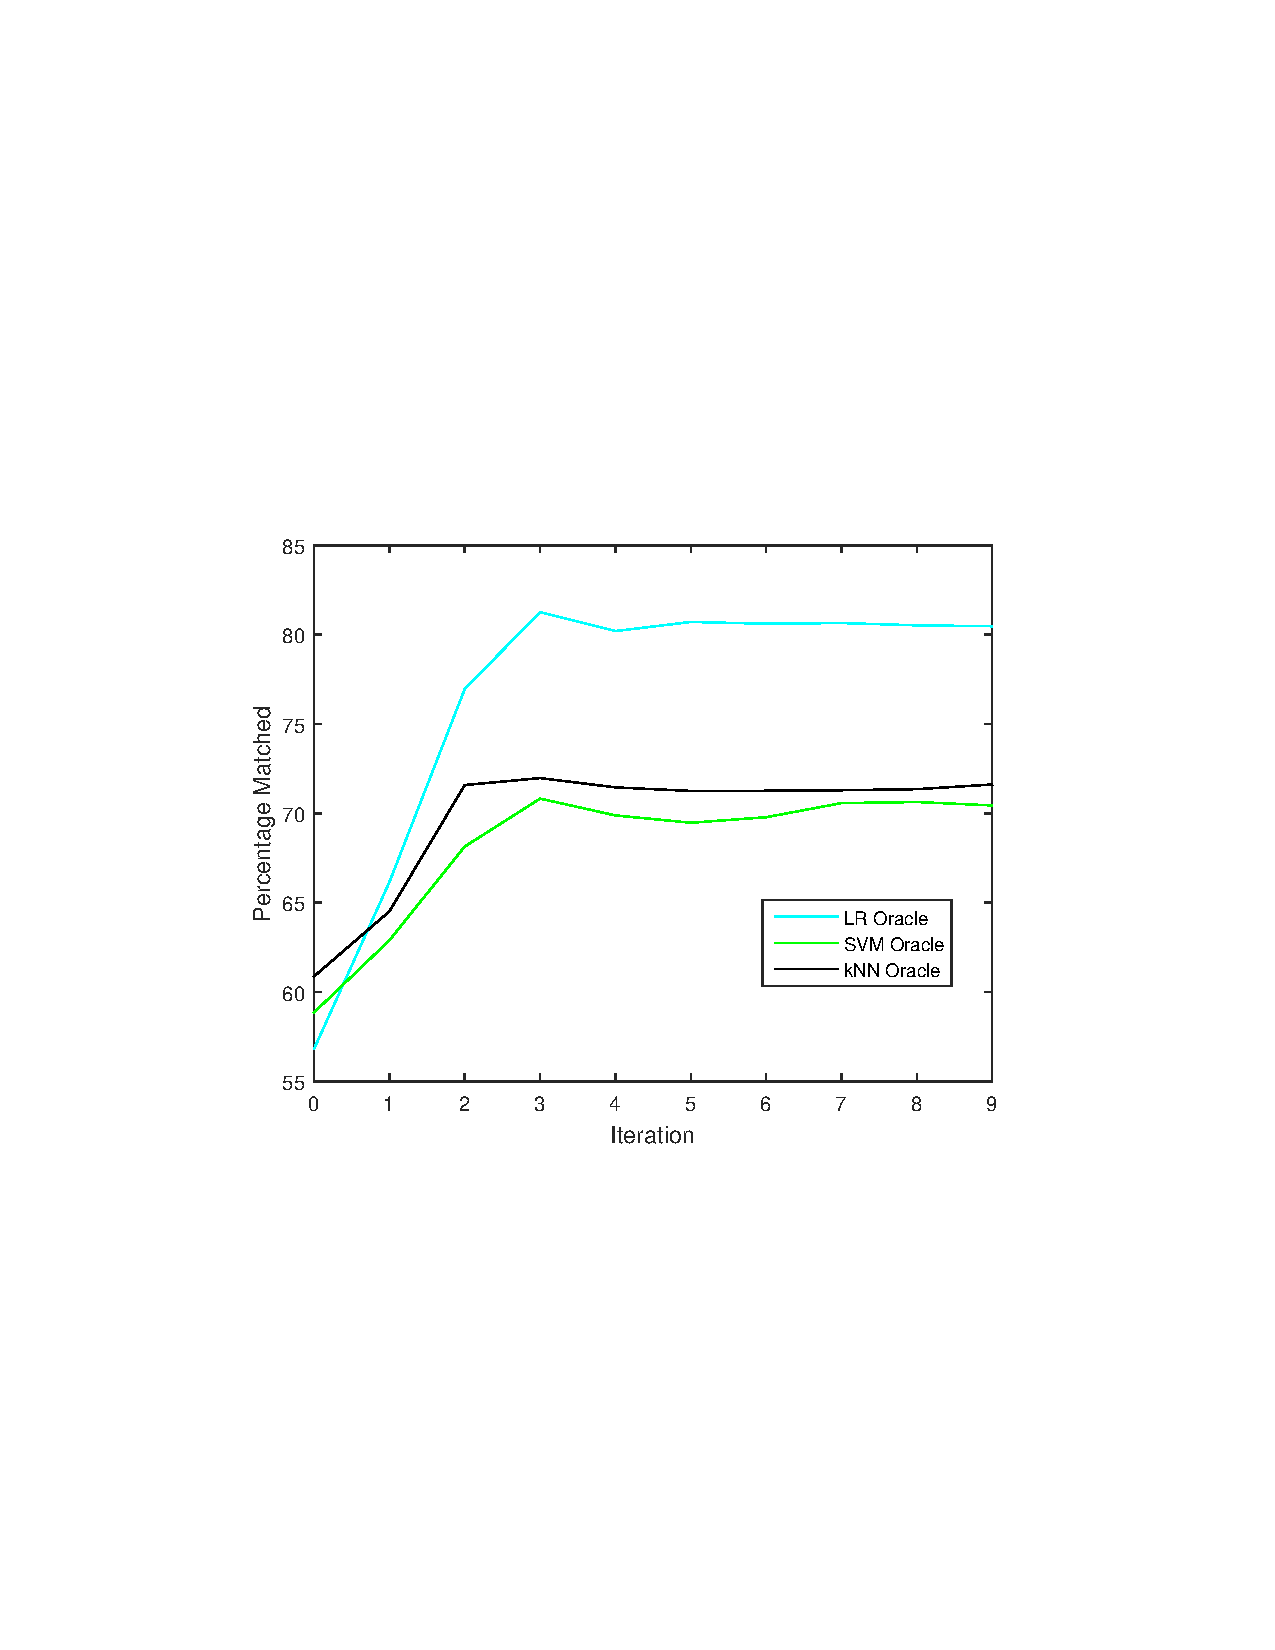
\includegraphics[width =\linewidth, trim = 110 240 120 255, clip]{figs/final_fig_1.pdf}
%		\caption{Percentage of samples for which the substitute model and oracle classifications agree without feature reduction.}
%		\label{fig:sub_approx}
%	\end{minipage}
%	\qquad
%	\begin{minipage}{0.42\linewidth}
%		\centering
%		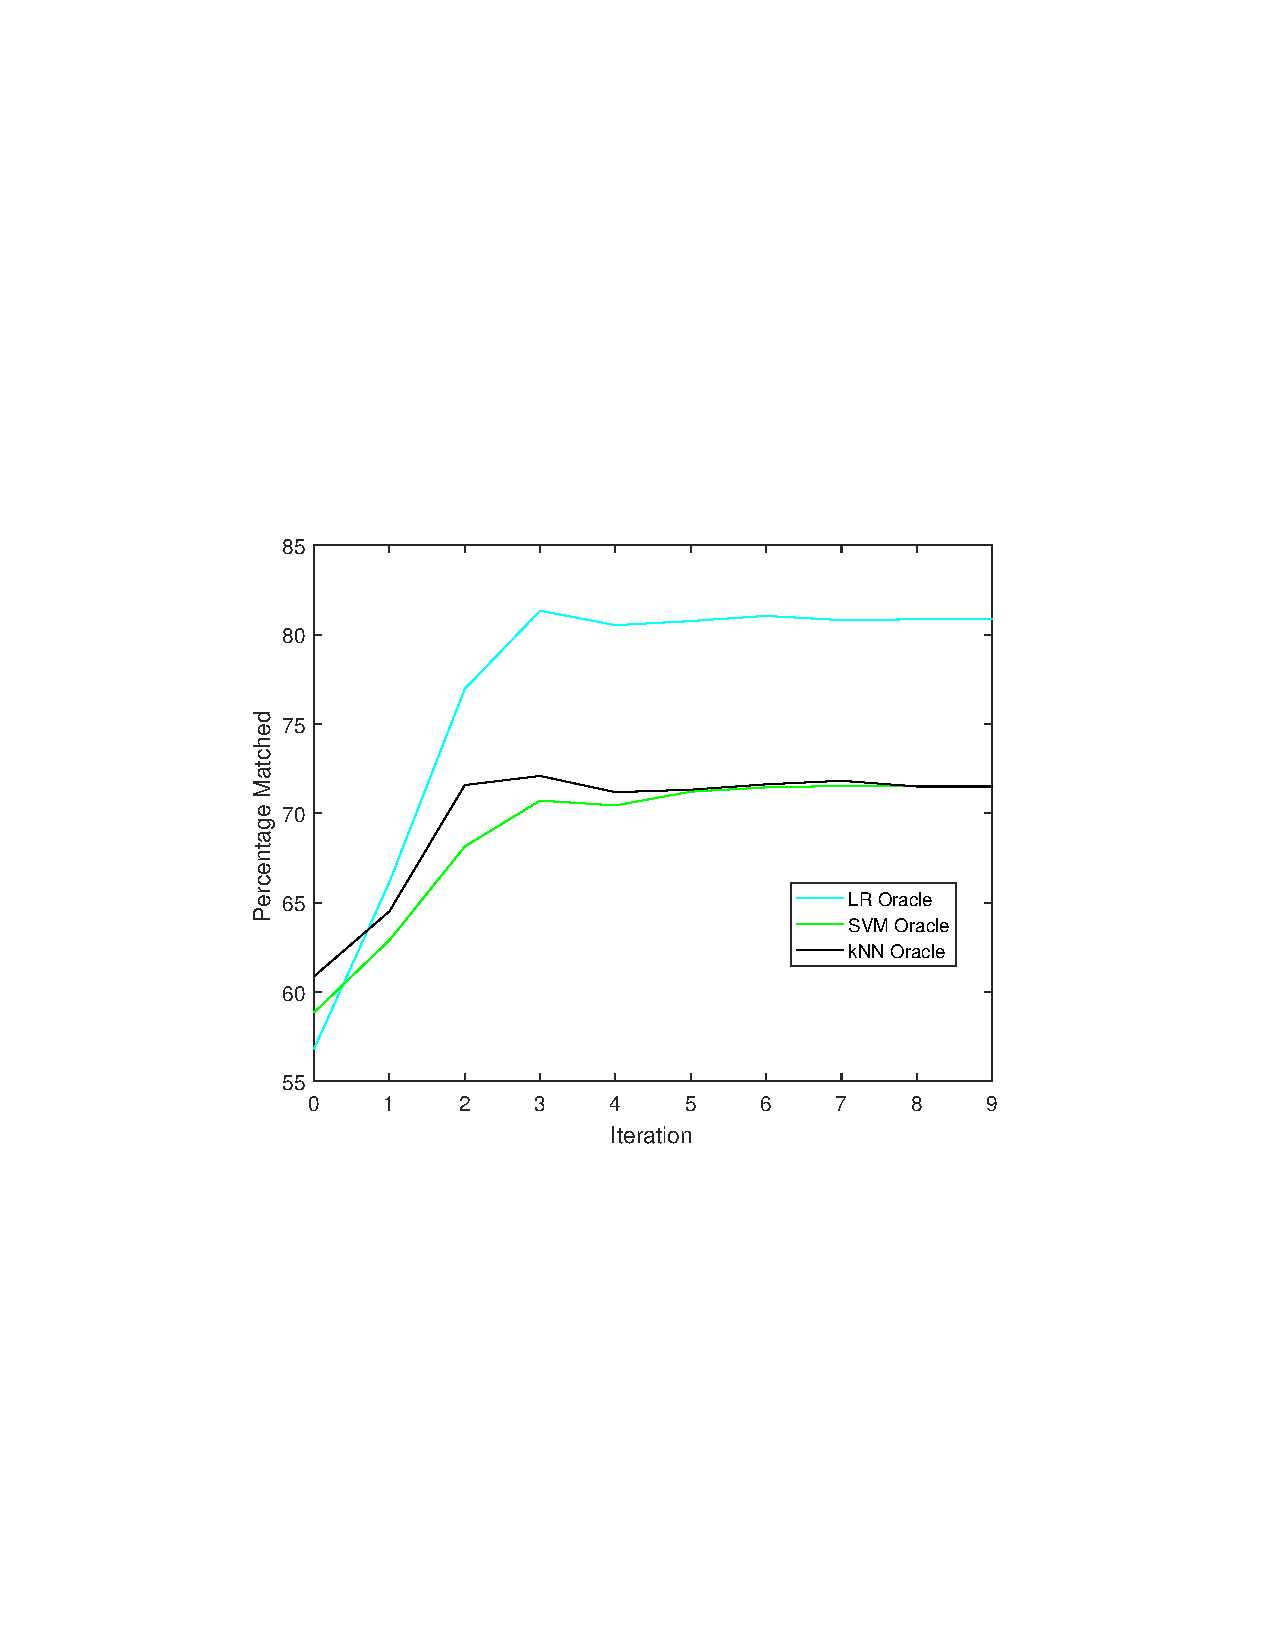
\includegraphics[width =\linewidth, trim = 110 240 120 255, clip]{figs/fig1_pca.pdf}
%		\caption{Percentage of samples for which the substitute model and oracle classifications agree with PCA feature reduction.}
%		\label{fig:sub_approx_pca}
%	\end{minipage}
%\end{figure*}

\begin{figure*}
	\centering
	\subfigure[Without feature reduction]{\label{fig:sub_approx}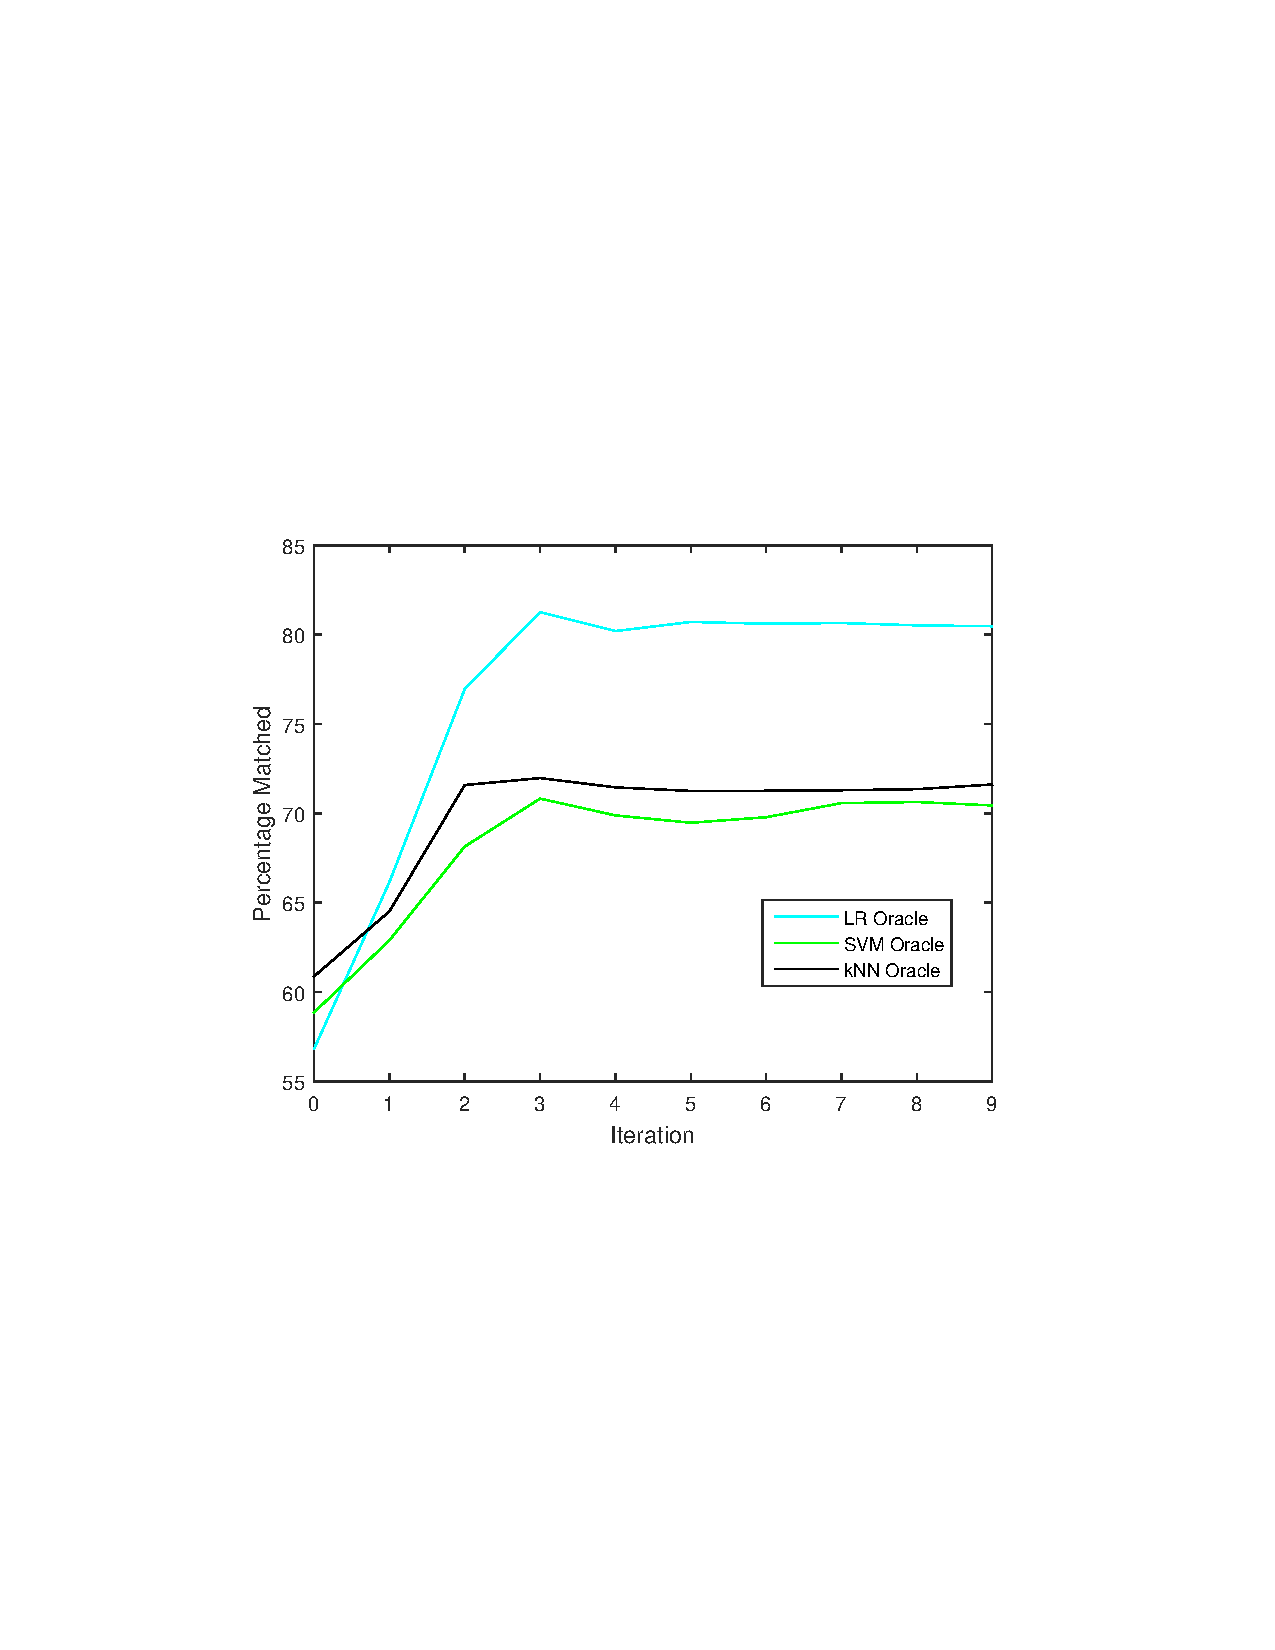
\includegraphics[width =0.415\linewidth, trim = 110 240 120 255, clip]{figs/final_fig_1.pdf}}
	\qquad
	\subfigure[With PCA feature reduction]{\label{fig:sub_approx_pca}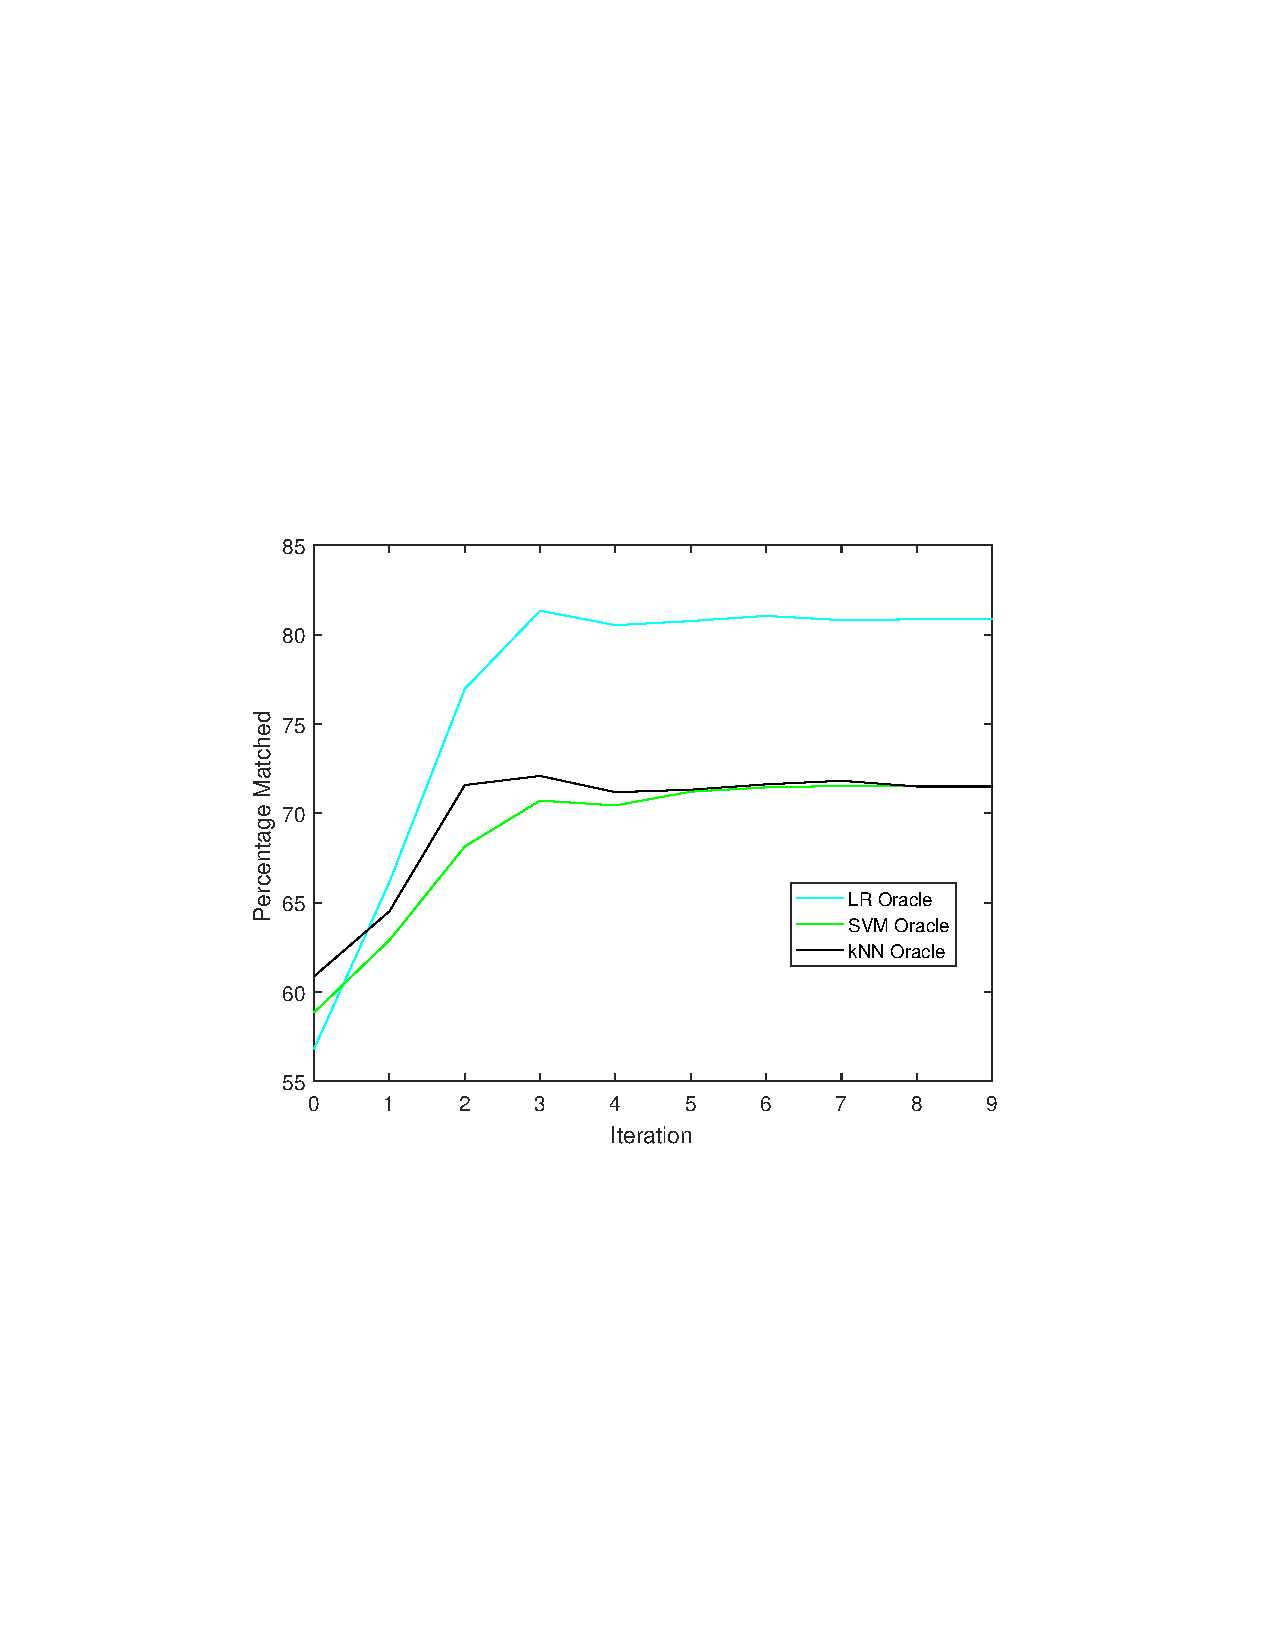
\includegraphics[width =0.415\linewidth, trim = 110 240 120 255, clip]{figs/fig1_pca.pdf}}
	\caption{Percentage of samples for which the substitute model and oracle classifications agree.}
\end{figure*}

\begin{figure*}
	\centering
	\subfigure[Fast Gradient Descent Algorithm]{\label{fig:missclassify_fgs}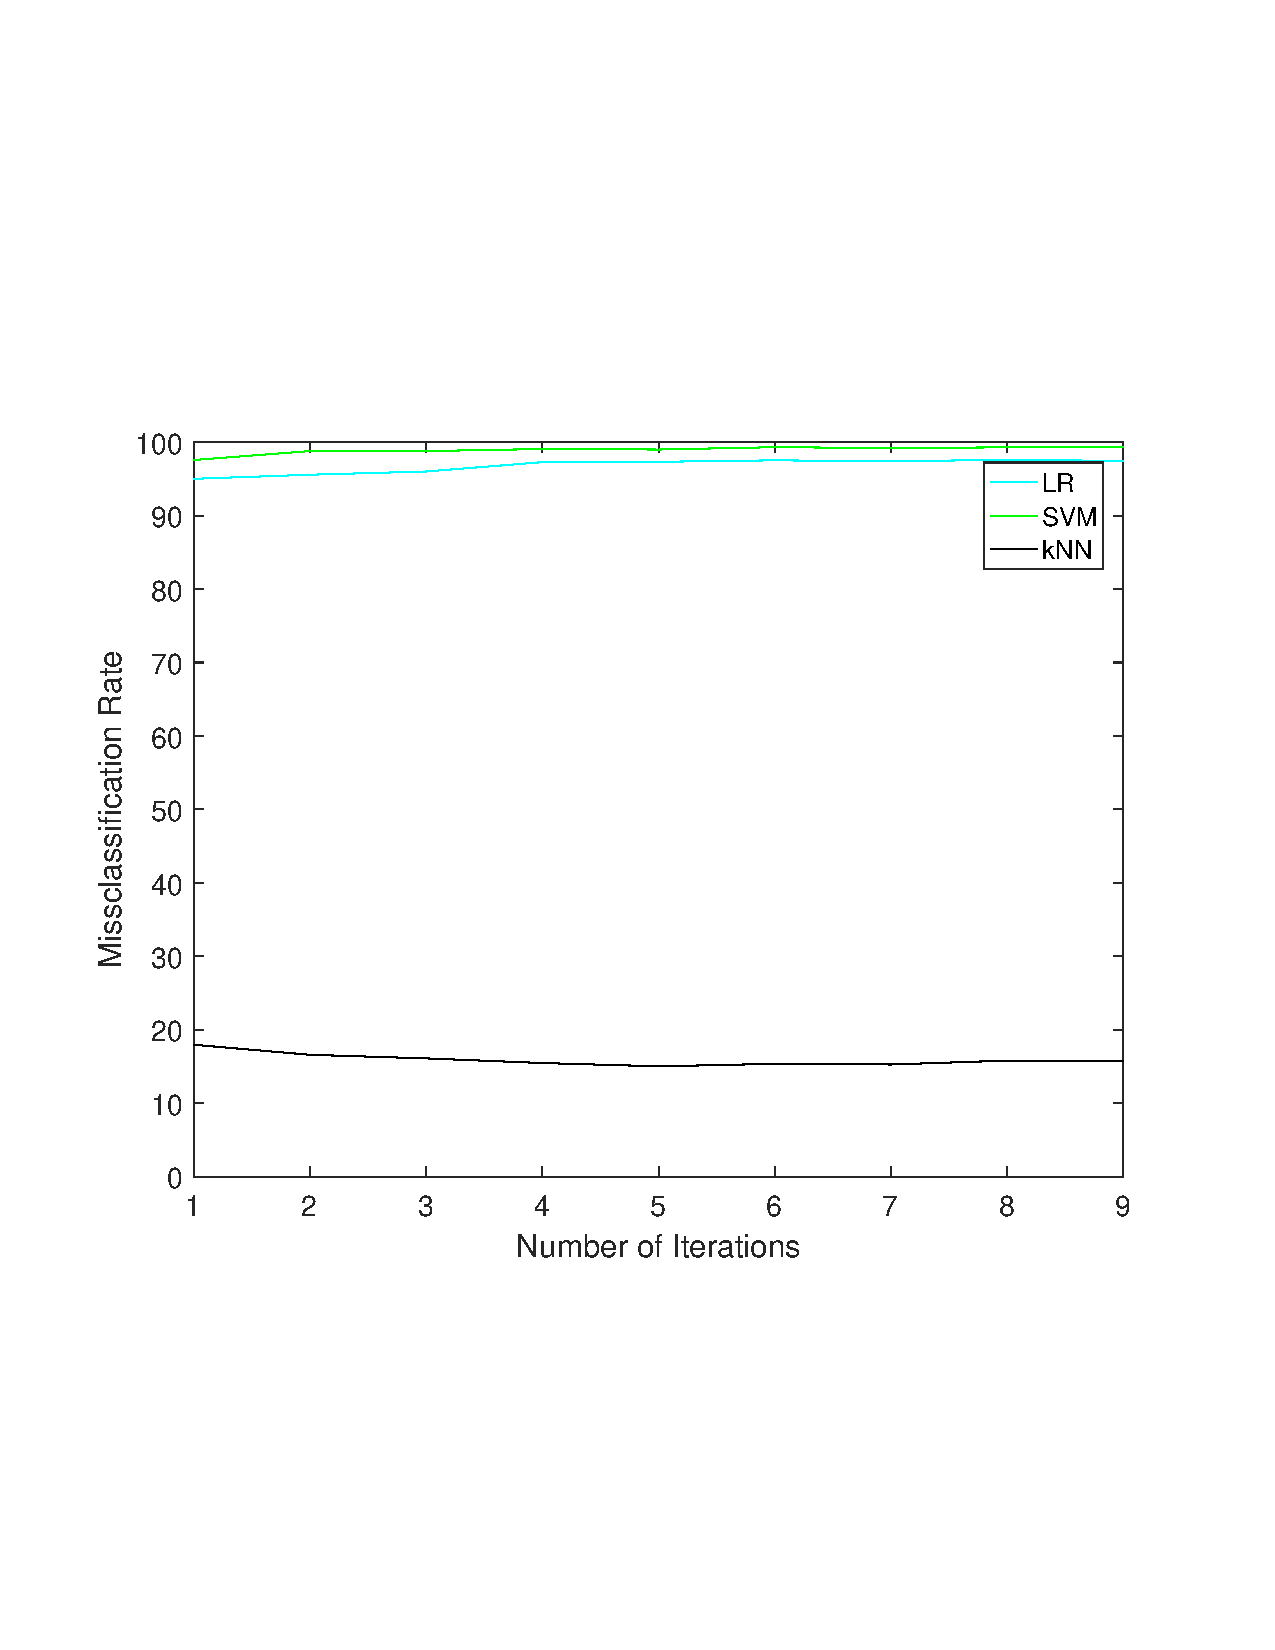
\includegraphics[width =0.4\linewidth, trim = 50 180 70 205, clip]{figs/misclass_goodfellow.pdf}}
	\qquad
	\subfigure[Papernot Algorithm]{\label{fig:missclassify_papernot}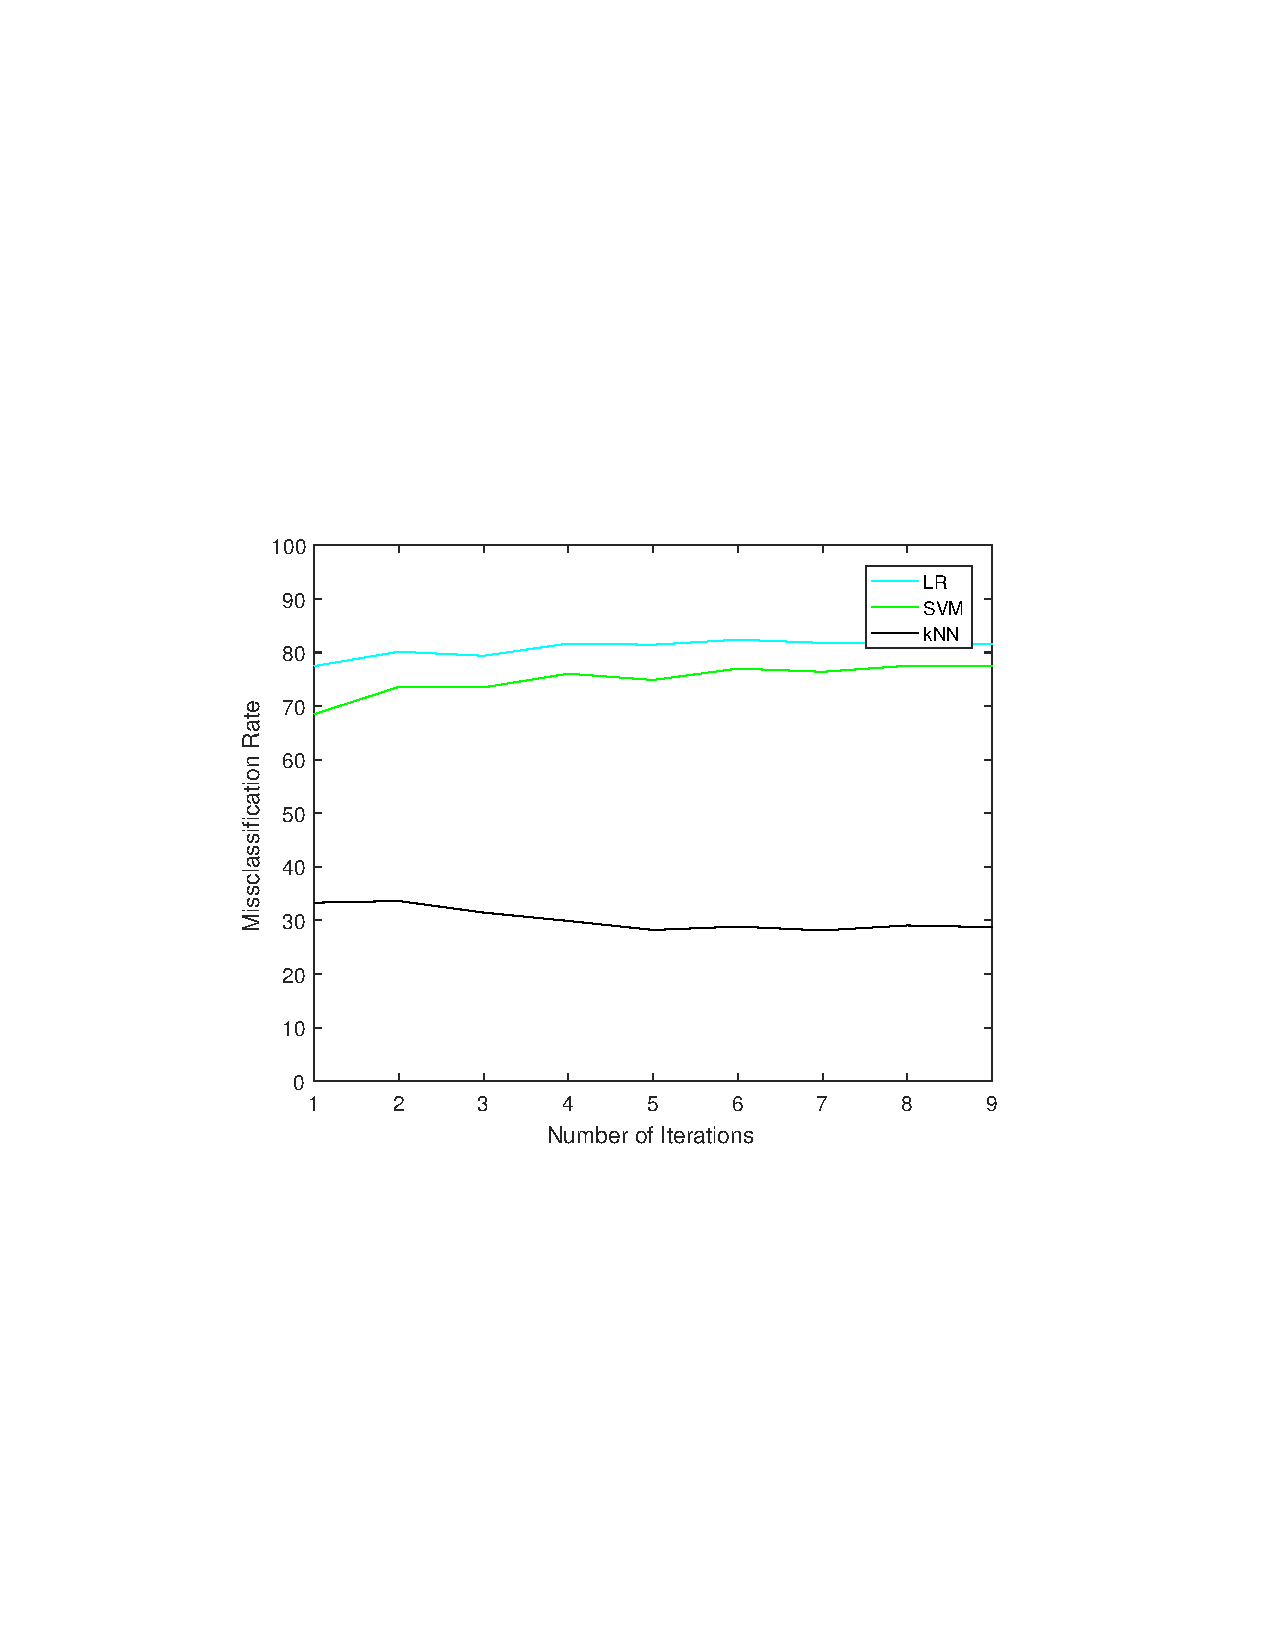
\includegraphics[width =0.415\linewidth, trim = 110 240 120 255, clip]{figs/missclass_papernot.pdf}}
	\caption{Misclassification rate vs. iteration of the Jacobian-based dataset augmentation without feature reduction.}
\end{figure*}

\begin{figure*}
	\centering
	\subfigure[Fast Gradient Descent Algorithm]{\label{fig:missclassify_fgspca}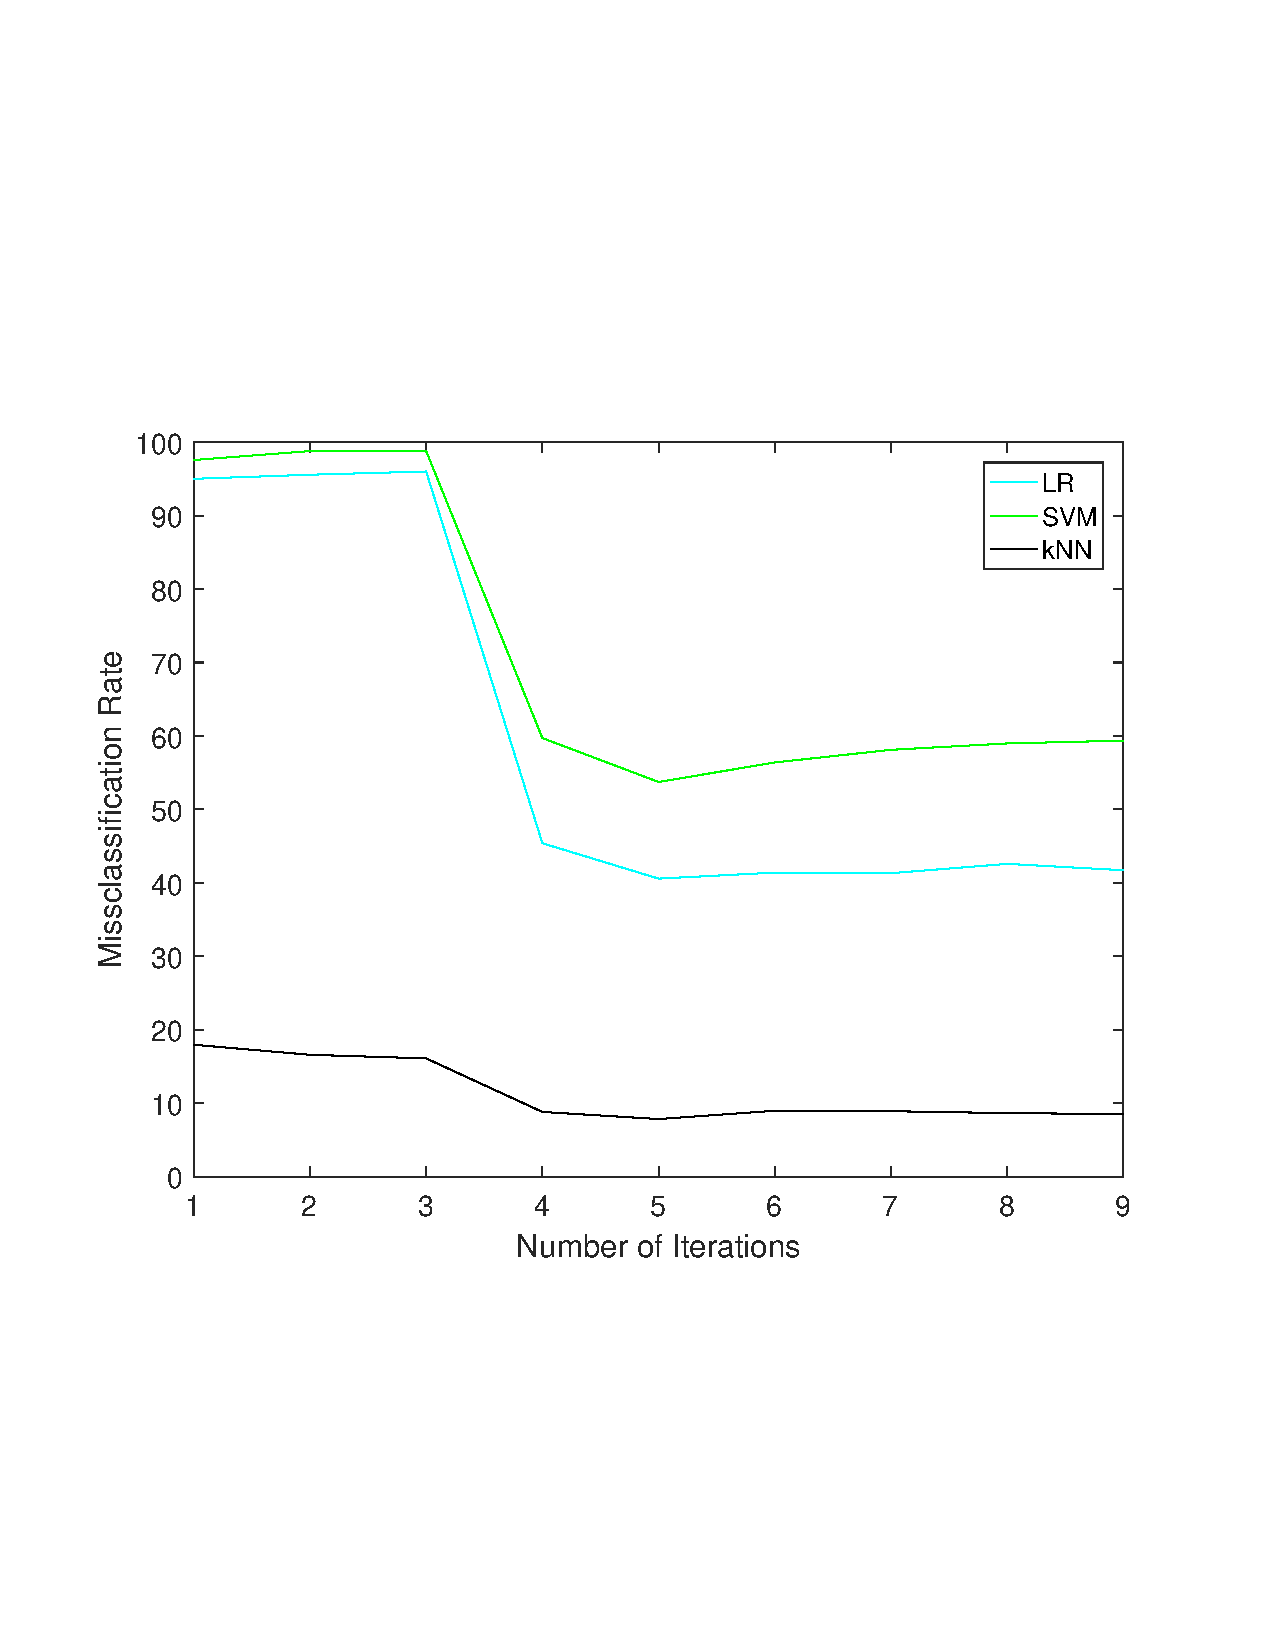
\includegraphics[width =0.4\linewidth, trim = 50 180 70 205, clip]{figs/misclass_goodfellow_pca.pdf}}
	\qquad
	\subfigure[Papernot Algorithm]{\label{fig:missclassify_papernotpca}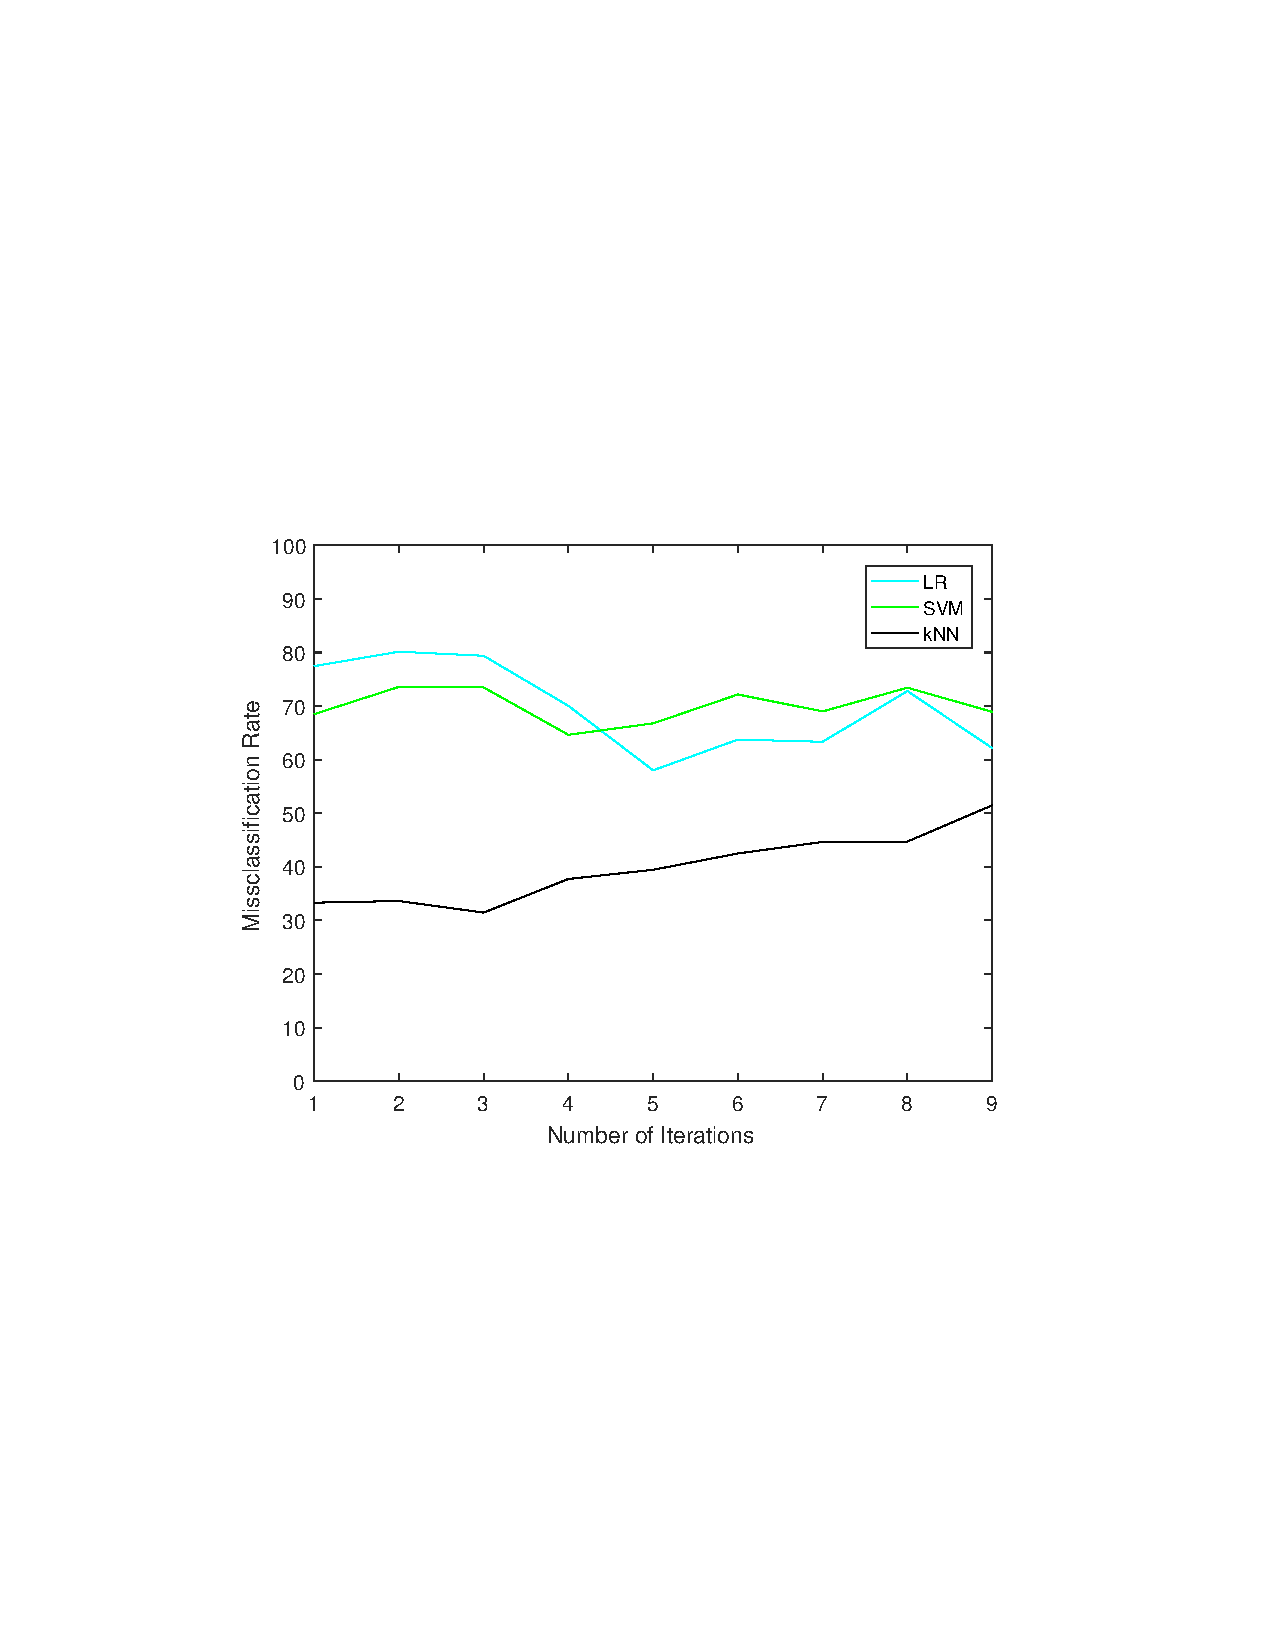
\includegraphics[width =0.415\linewidth, trim = 110 240 120 255, clip]{figs/missclass_papernot_pca.pdf}}
	\caption{Misclassification rate vs. iteration of the Jacobian-based dataset augmentation with PCA feature reduction.}
\end{figure*}

A comparison of the success of the LR substitute model against the oracle with PCA feature reduction is portrayed in Figure \ref{fig:sub_approx_pca}. The PCA algorithm reduced the dimensionality of the feature space by a factor of 8, but the results of the trained LR substitute model were nearly identical to those with the entire feature space. Hence, PCA has minimal effect on the training of the substitute model, and is a valid method for feature space reduction. 

\subsection{Performance of Crafted Adversarial Samples}
In our first experiment, we generated adversarial samples on the $10,000$ test samples based on the LR substitute model. The misclassification rates on the adversarial samples by the oracles are given in Figures \ref{fig:missclassify_fgs}  and \ref{fig:missclassify_papernot} for both the FGS and Papernot methods utilizing the full feature sets. To generate adversarial samples with FGS, we used $\epsilon = 0.3$ in Equation $\ref{eqn:fast_gradient_sign}$, which is the same value as that used in $\cite{papernot3}$. For the Papernot method, $10\%$ of the features (pixels) were perturbed for each image ($\gamma = 0.1$) with $\epsilon = 1$, similar to the parameters in \cite{papernot1}. \\
\indent In Figures \ref{fig:missclassify_fgs}  and \ref{fig:missclassify_papernot}, we were able to achieve fairly high misclassification rates for both the LR oracle and the SVM oracle, but performed poorly for the kNN oracle, which agrees with the results obtained by Papernot et al. $\cite{papernot3}$. Our misclassification rate was, in fact, slightly higher for all 3 models for the FGS method as reported in \cite{papernot3}, likely caused by the different gradient formulation utilized in our approach. The Papernot method performed notably worse than FGS due to intrinsically smaller perturbations. However, the Papernot parameters can be further tuned to achieve a desired balance between the misclassification rate and the amount of perturbation.\\
\indent In our second experiment, PCA feature-reduction was introduced at iteration 4 of the Jacobian-based dataset augmentation, when the training set size exceeded the number of features. Adversarial samples were generated by first carrying out FGS and Papernot algorithms on the reduced feature space and then restoring the samples as described in section \ref{sec:pca} before passing them into the oracle. The results are shown in Figures \ref{fig:missclassify_fgspca} and \ref{fig:confusion_matrix_papernotpca}. From Figure \ref{fig:missclassify_fgspca}, we can see that introducing PCA in the FGS algorithm dramatically decreased the misclassification rate. However, from Figure \ref{fig:missclassify_papernotpca}, the misclassification rate for the Papernot algorithm was only slightly impacted by the introduction of PCA, maintaining a reasonable misclassification rate of about $\sim 70\%$. For the kNN oracle, the rate even increased according to the figure. This suggests that PCA is a suitable feature reduction technique to use for the Papernot algorithm, specifically.\\
\indent To calculate the computational cost, we measured the time required to generate all $10,000$ of the adversarial samples in both experiments. The results are shown in Table \ref{tablewithstuff}. For the FGS algorithm, although there was a reduction in running time, the change was not significant, as FGS is already computationally efficient. For the Papernot algorithm, the reduction was substantial; the running time was cut by more than a factor of 2 for all three oracles. This suggests that PCA is successful at reducing the computational cost associated with the Papernot algorithm.\\
\indent The confusion matrices for the unaltered test images and the adversarial samples generated using the Papernot algorithm with PCA are shown in Figures \ref{fig:confusion_matrix_oracle} and \ref{fig:confusion_matrix_papernotpca}, respectively. The number in position $(i, j)$ of the grid corresponds to the percentage of class $i$ images being classified as class $j$. The Papernot algorithm with PCA was generally successful at misdirecting the oracle, except for the numbers "1" and "6" (darker squares in Figure \ref{fig:confusion_matrix_papernotpca}), which were robust to the attack. The precision, recall, and accuracy for all test samples and adversarial samples are displayed in Table \ref{tablewithstuff}, presenting the same trends as in the confusion matrices.\\
\indent A single unaltered image and its associated sample adversarial images are shown in Figure \ref{fig:picof9s}. Both the SVM oracle and the LR oracle misclassified the perturbed images. We can see that these images are still easily recognizable as a "9", so the adversarial attacks were successful. However, the deviations added to the image are also clearly visible to the human eye, which is undesirable. These deviations could be reduced with further parameter tuning and higher resolution images. Note that, as expected, the deviations added to the image were less noticeable in the Papernot algorithm as compared to that of the FGS method. 

%This explains why Papernot algorithm was found to have a lower misclassification rate than FGS algorithm.

%We implemented the above algorithm utilizing a reduced image feature set. Specifically, we reduced each of the $28 \times 28$ pixel images in the LR substitute model training set by a \textbf{factor of 8}.

\begin{figure*}[h]
	\centering
	\begin{minipage}{0.45\linewidth}
		\centering
		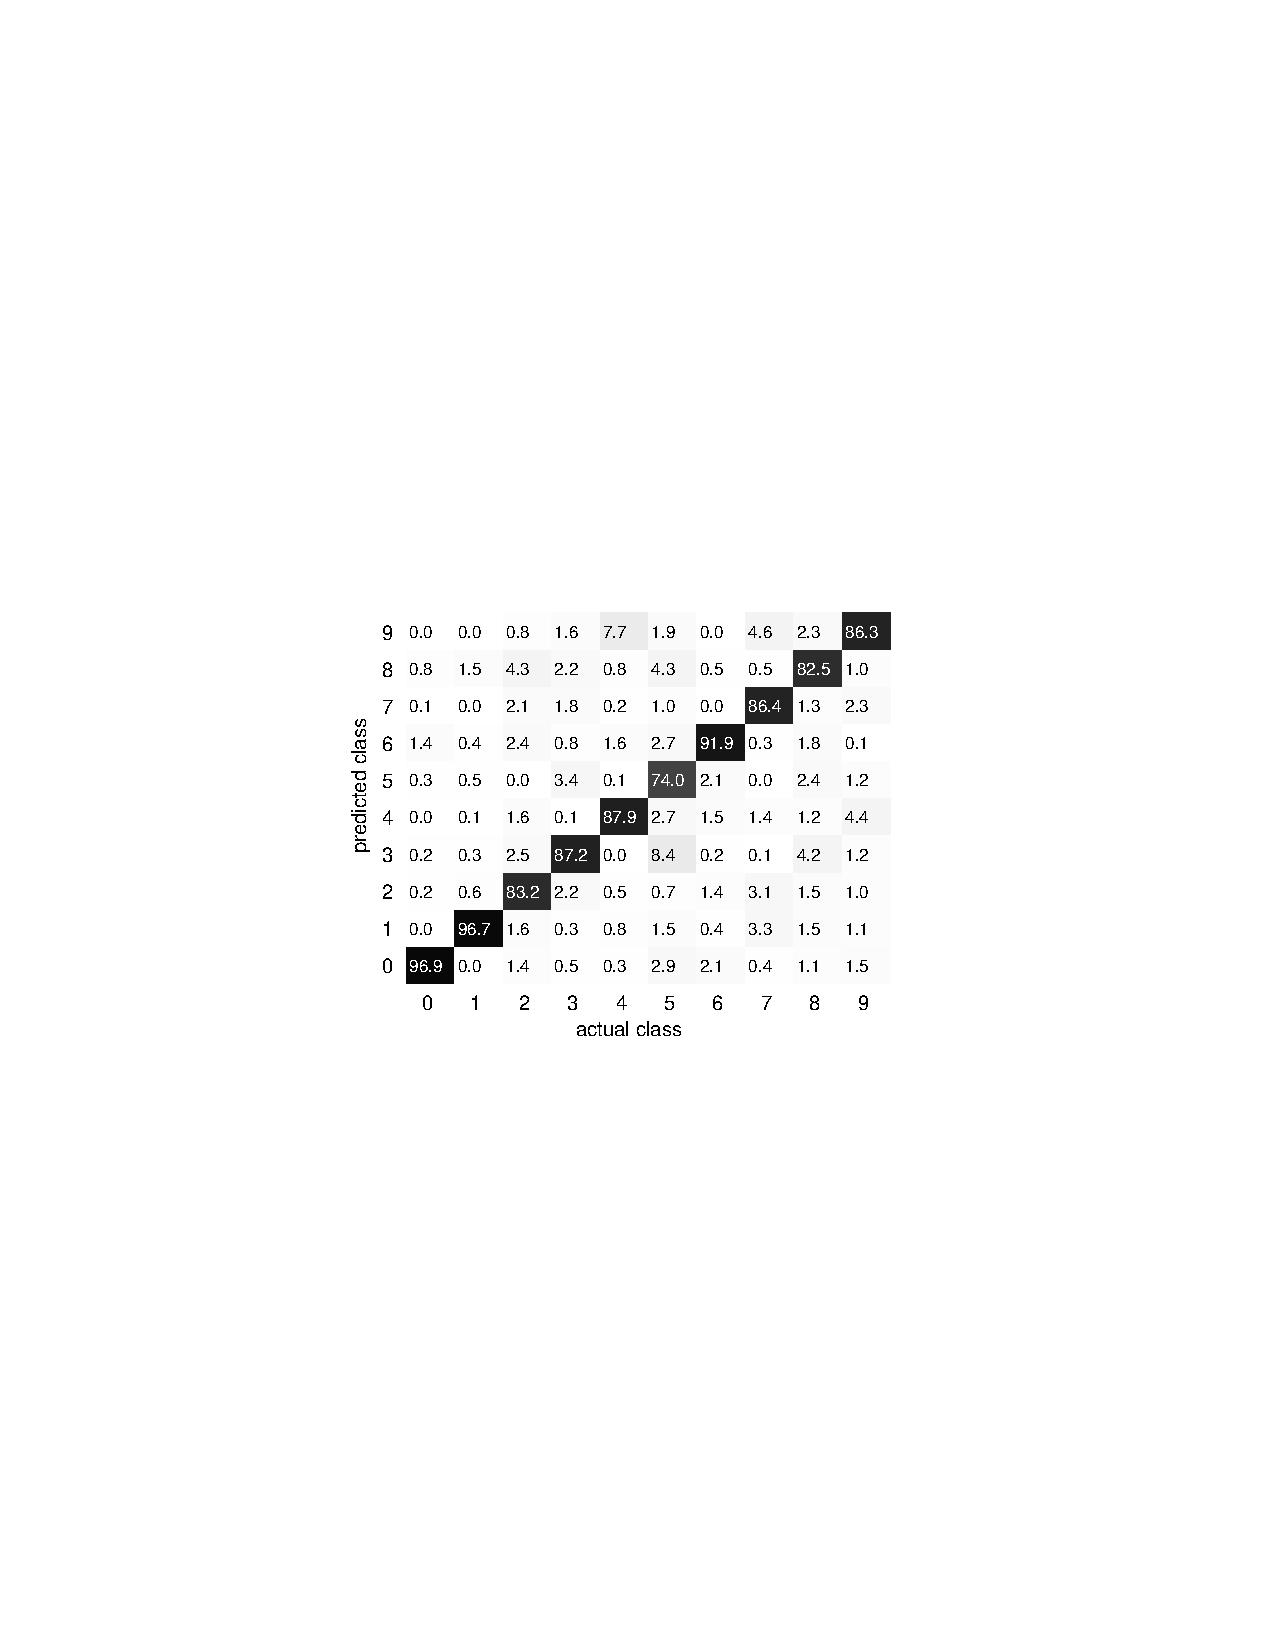
\includegraphics[width =\linewidth, trim = 140 295 150 280, clip]{figs/confusion_matrix_oracle.pdf}
		\caption{Confusion matrix against the LR oracle for the original 10,000 test samples.}
		\label{fig:confusion_matrix_oracle}
	\end{minipage}
	\qquad
	\begin{minipage}{0.45\linewidth}
		\centering
		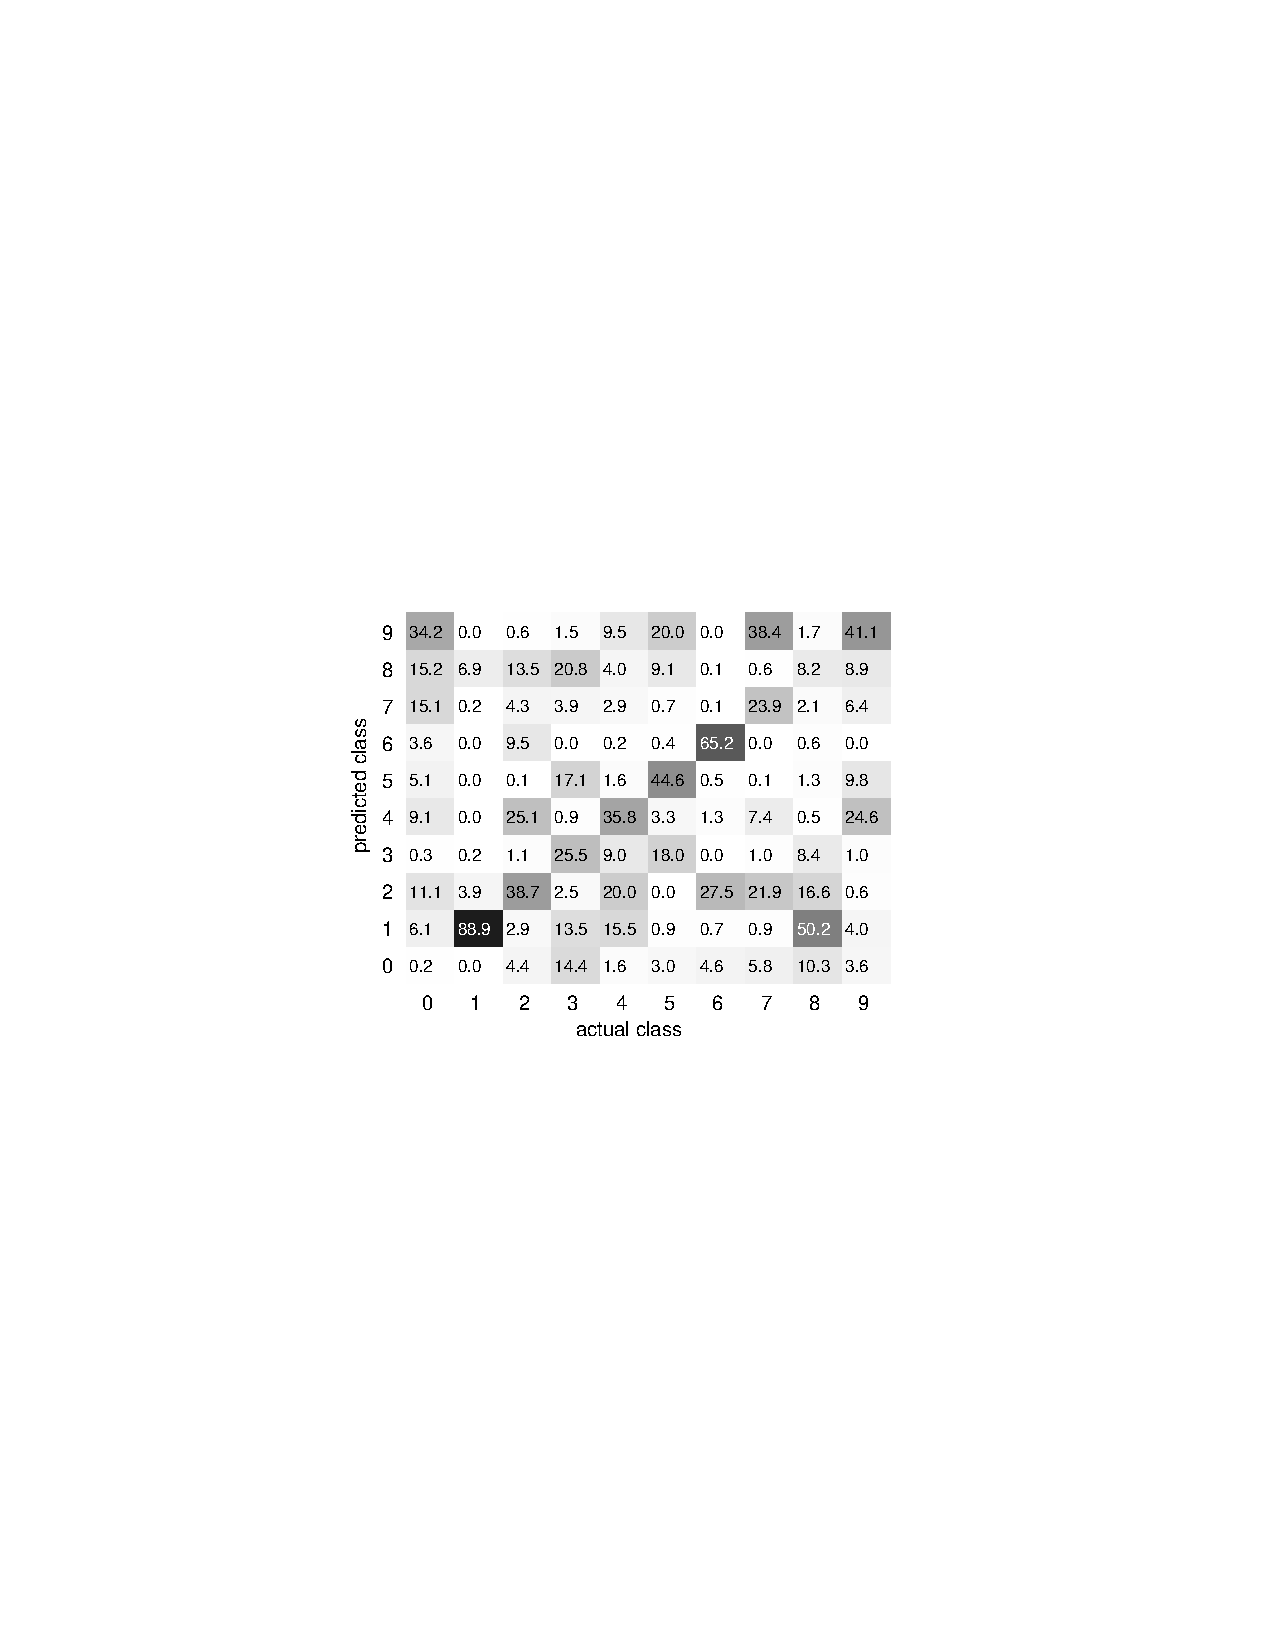
\includegraphics[width =\linewidth, trim = 140 295 150 265, clip]{figs/confusion_matrix_papernotpca.pdf}
		\caption{Confusion matrix against the LR oracle for the 10,000 adversarial samples generated using the Papernot method with PCA.}
		\label{fig:confusion_matrix_papernotpca}
	\end{minipage}
\end{figure*}

\begin{table}[t]
	\caption{Runtime for generating 10,000 adversarial samples in seconds for the three oracle models using FGS.}
	\label{runtime_FGS}
	\vskip 0.15in
	\begin{center}
		\begin{small}
			\begin{sc}
				\begin{tabular}{lccr}
					\hline
					\abovespace\belowspace
					&LR & SVM & kNN\\
					\hline
					\abovespace
					FGS & 1.3912 & 1.5692 & 1.7441 \\
					FGS + PCA & 1.3509 & 1.2557 & 1.3681\\				
					\hline
				\end{tabular}
			\end{sc}
		\end{small}
	\end{center}
	\vskip -0.1in
\end{table}

\begin{table}[t]
	\caption{Runtime for generating 10,000 adversarial samples in seconds for the three oracle models using Papernot method.}
	\label{runtime_Papernot}
	\vskip 0.15in
	\begin{center}
		\begin{small}
			\begin{sc}
				\begin{tabular}{lccr}
					\hline
					\abovespace\belowspace
					&LR & SVM & kNN\\
					\hline
					\abovespace
					Papernot & 7.9147 & 7.9776 & 8.57\\
					Papernot + PCA & 3.1826 & 3.0719 & 3.3997\\				
					\hline
				\end{tabular}
			\end{sc}
		\end{small}
	\end{center}
	\vskip -0.1in
\end{table}

\begin{table}[t]
	\caption{Average precision, recall, and accuracy for the original test images and adversarial images constructed using Papernot algorithm with PCA.}
	\label{tablewithstuff}
	\vskip 0.15in
	\begin{center}
		\begin{small}
			\begin{sc}
				\begin{tabular}{lccc}
					\hline
					\abovespace\belowspace
					&Precision & Recall & Accuracy\\
					\hline
					\abovespace
					Original & 87.4645 &  87.3036  & 87.5300 \\
					Adversarial & 37.3687 &  37.2288 &  37.8400\\				
					\hline
				\end{tabular}
			\end{sc}
		\end{small}
	\end{center}
	\vskip -0.1in
\end{table}

\begin{figure}[b]
\centering
\begin{minipage}{.09\textwidth}
	\centering
    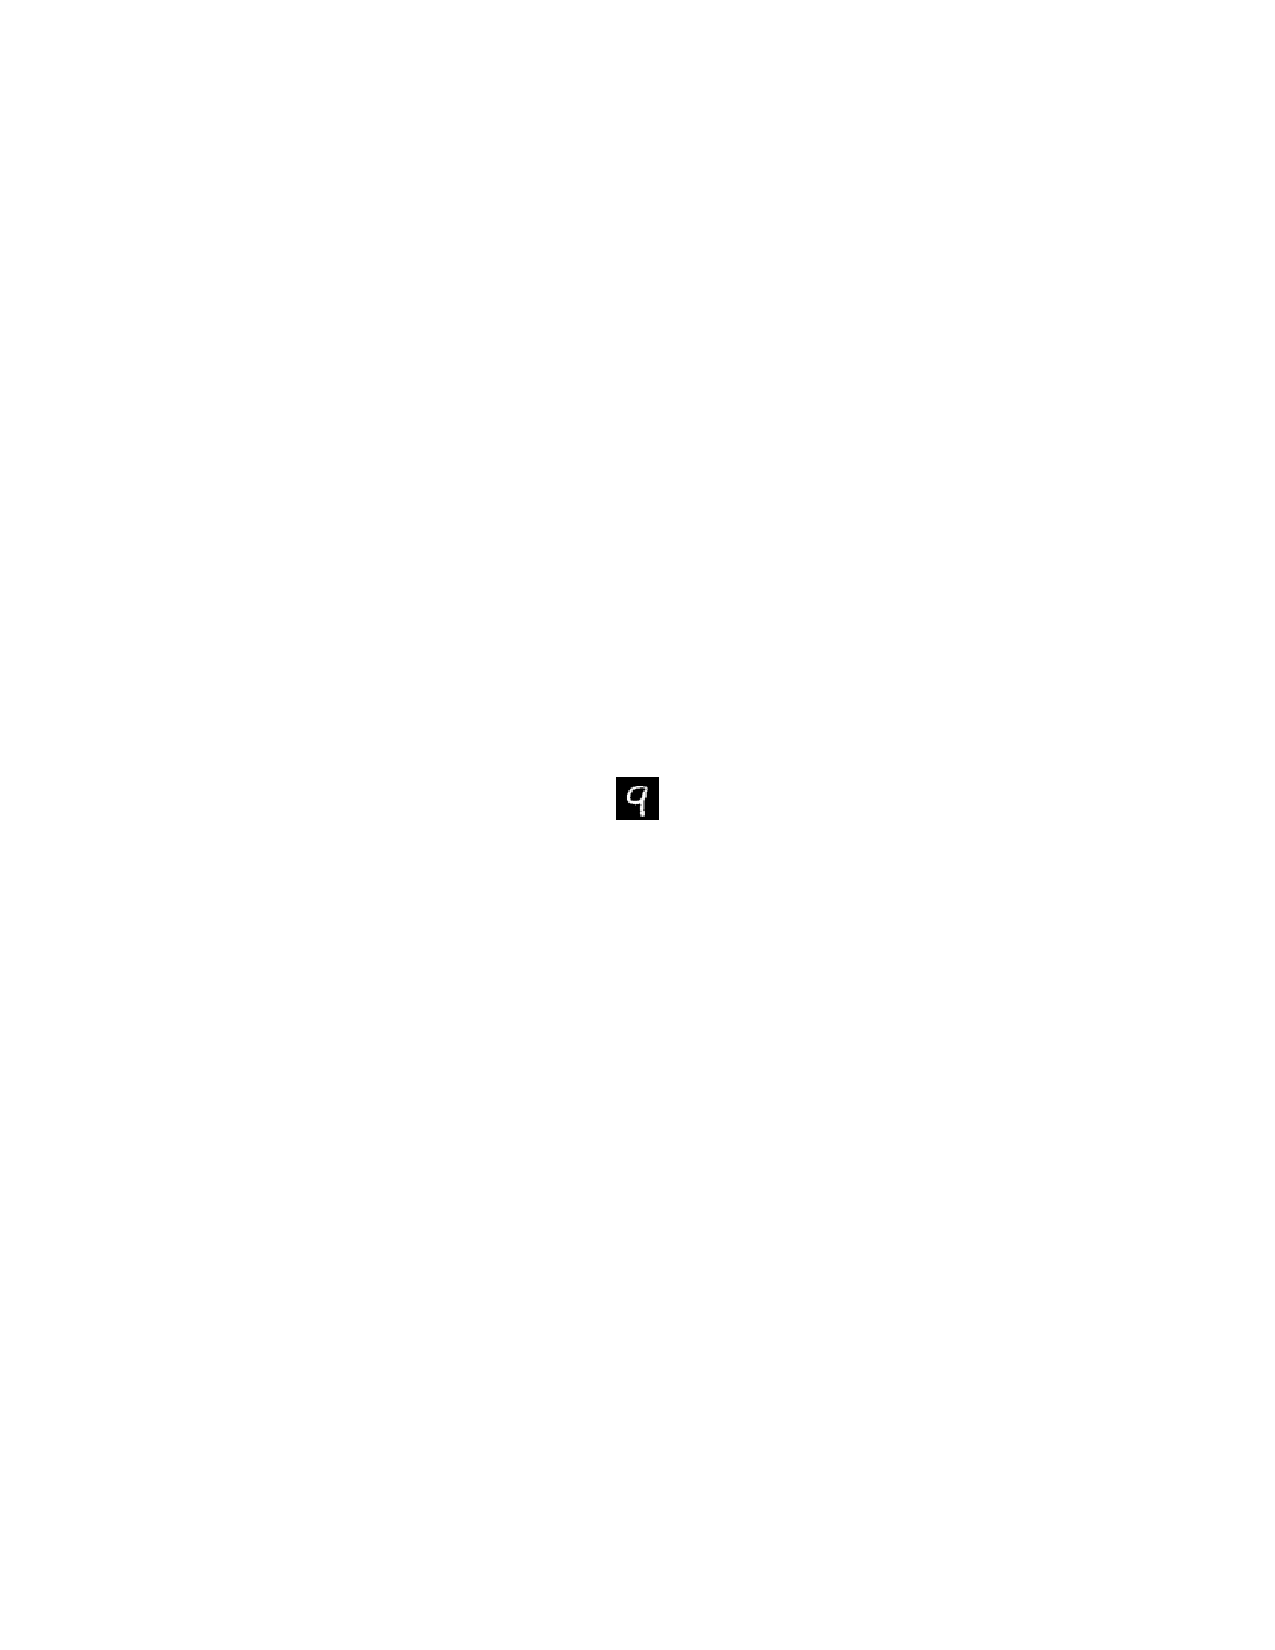
\includegraphics[width =0.9\linewidth, trim = 300 400 300 375, clip]{figs/orig9.pdf}
\end{minipage}%
\begin{minipage}{.09\textwidth}
	\centering
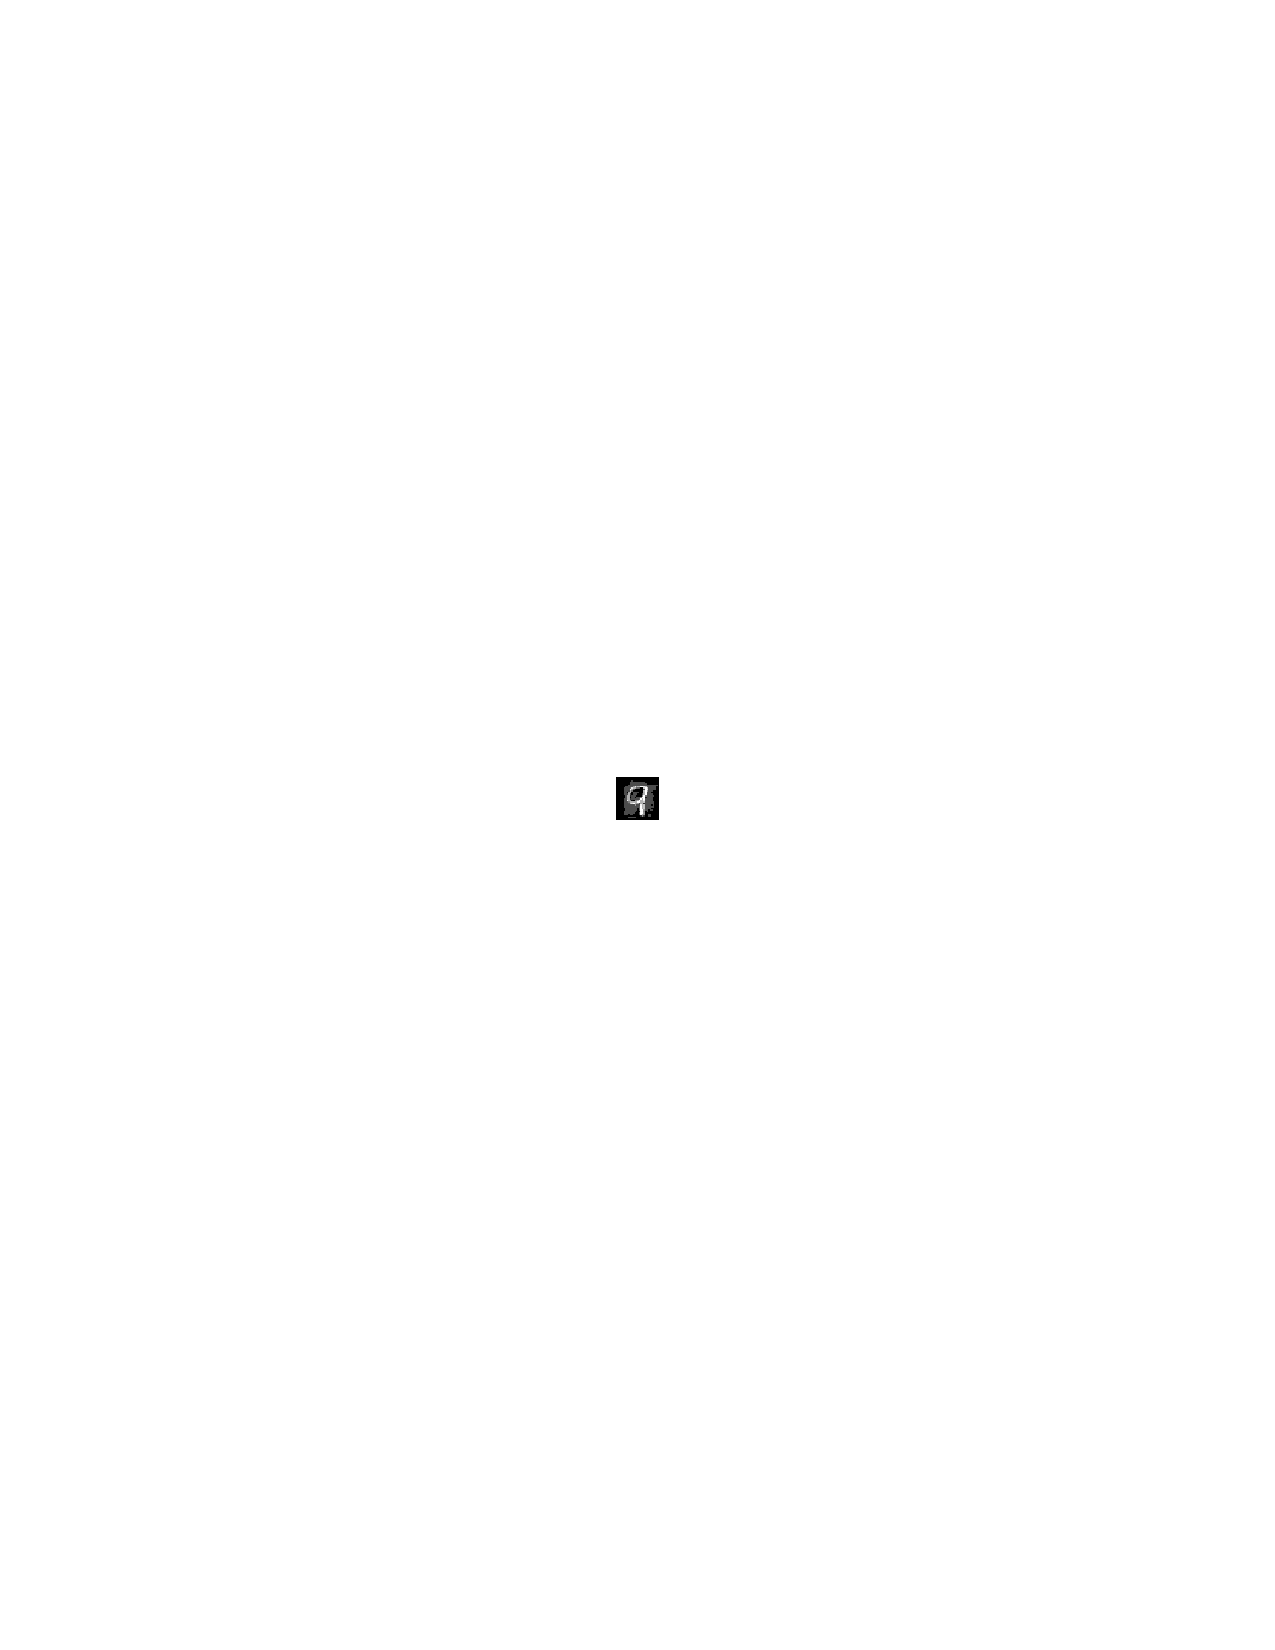
\includegraphics[width =0.9\linewidth, trim = 300 400 300 375, clip]{figs/goodfellow9.pdf}
\end{minipage}
\begin{minipage}{.09\textwidth}
	\centering
    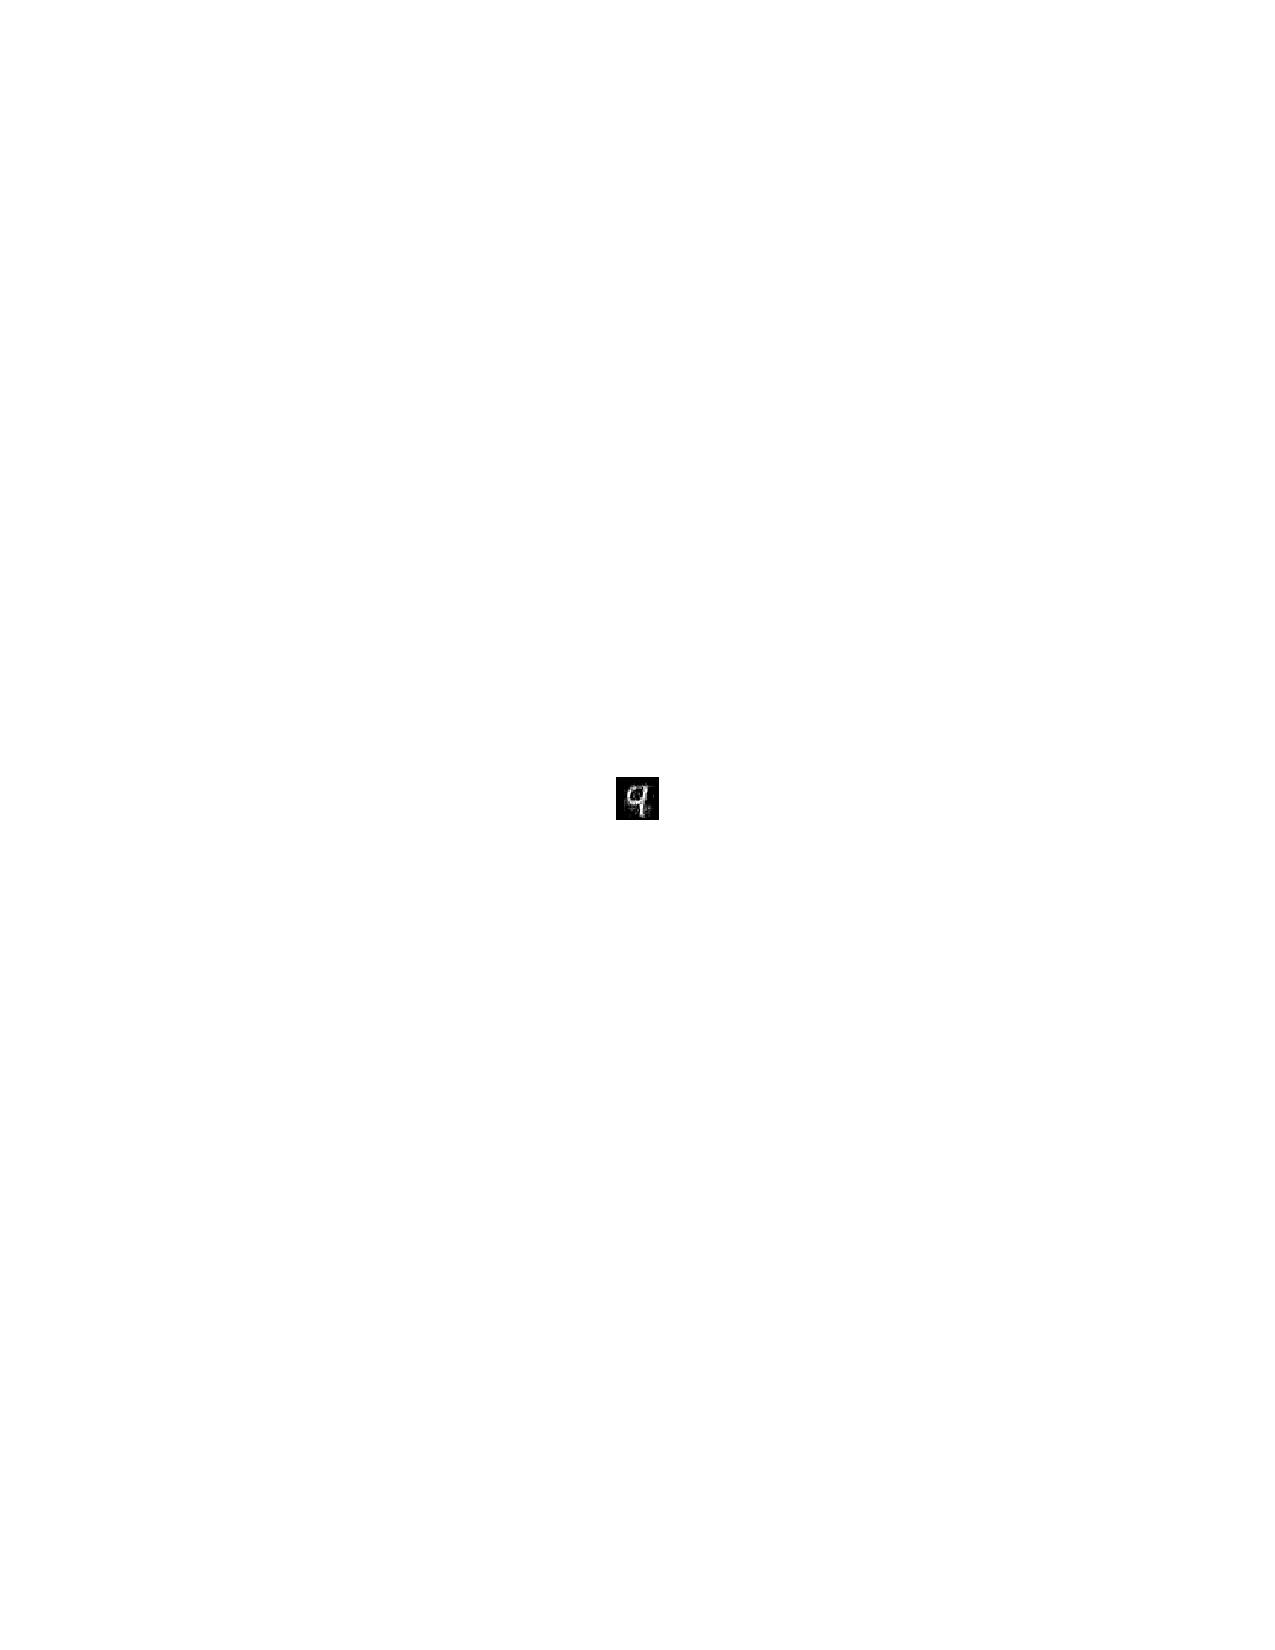
\includegraphics[width =0.9\linewidth, trim = 300 400 300 375, clip]{figs/goodfellow9pca.pdf}
\end{minipage}
\begin{minipage}{.09\textwidth}
	\centering
    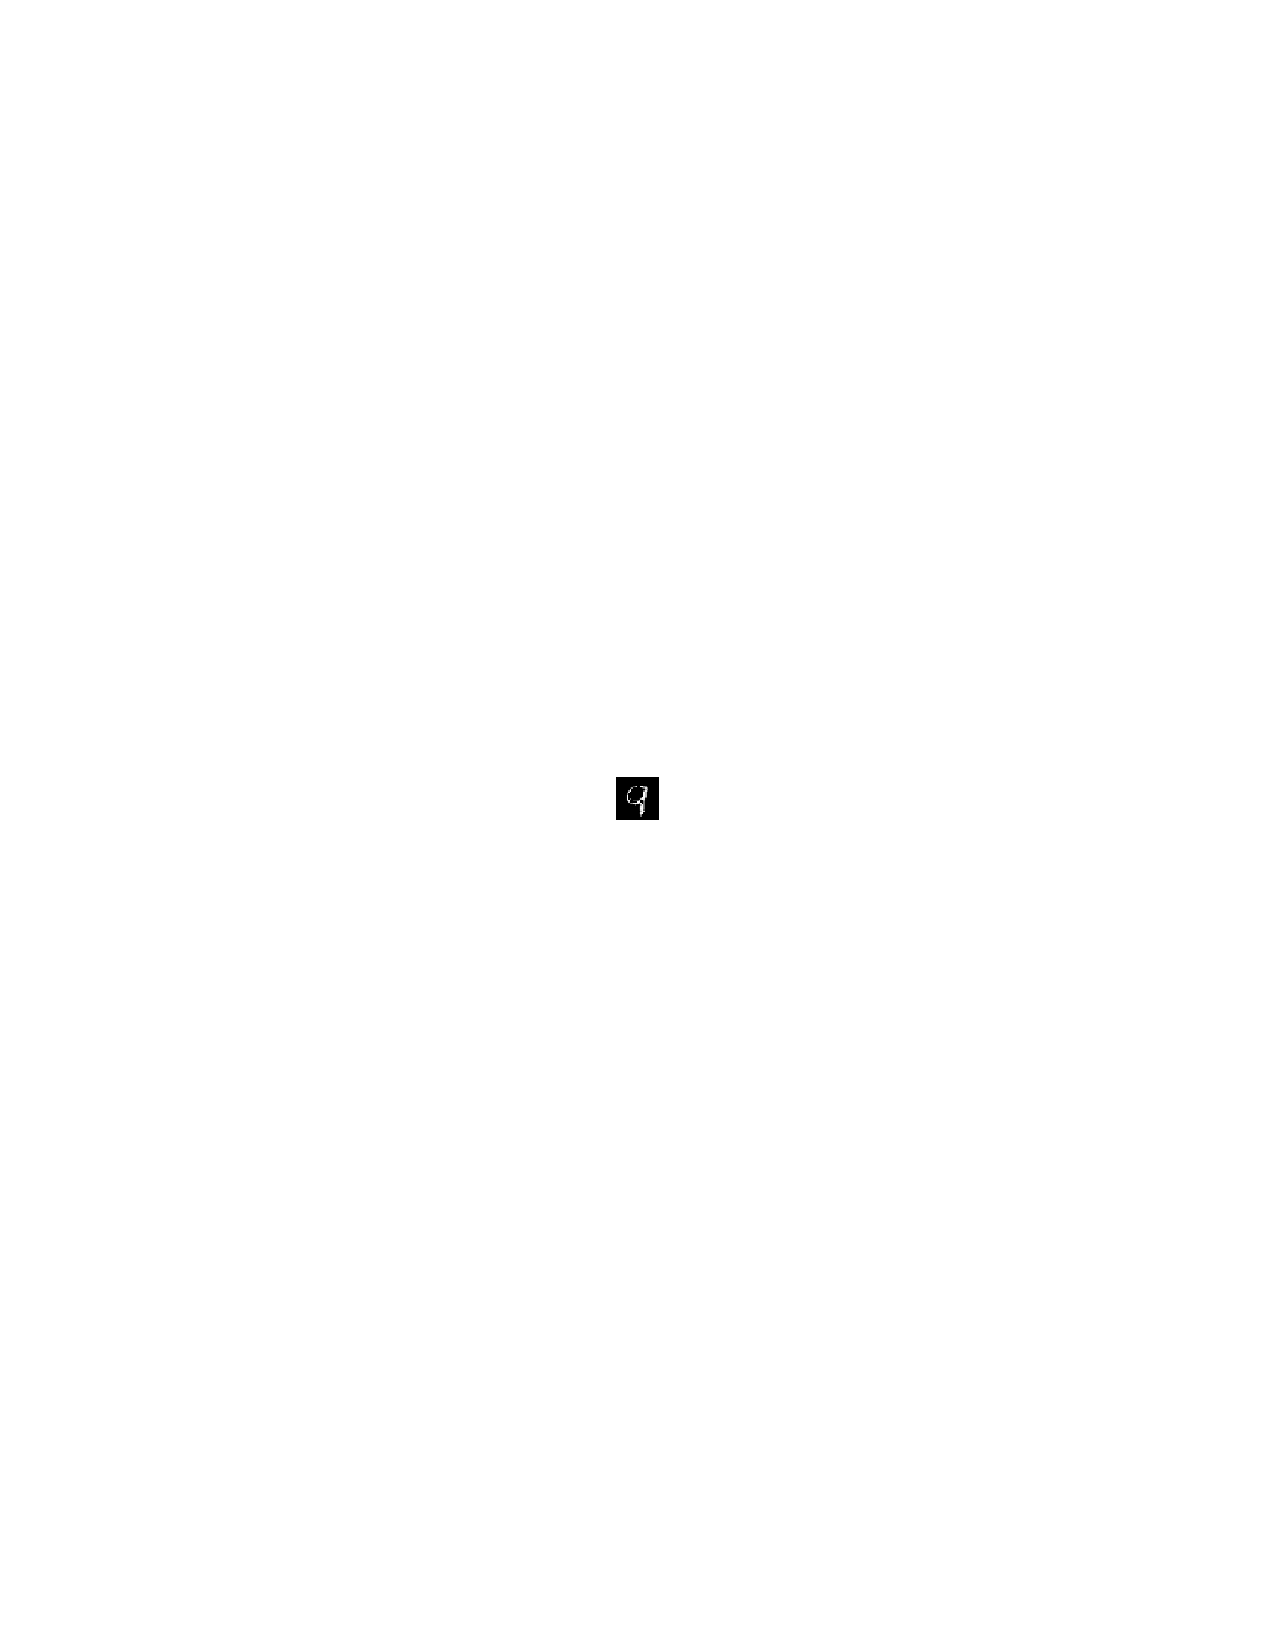
\includegraphics[width =0.9\linewidth, trim = 300 400 300 375, clip]{figs/papernot9.pdf}
\end{minipage}
\begin{minipage}{.09\textwidth}
	\centering
    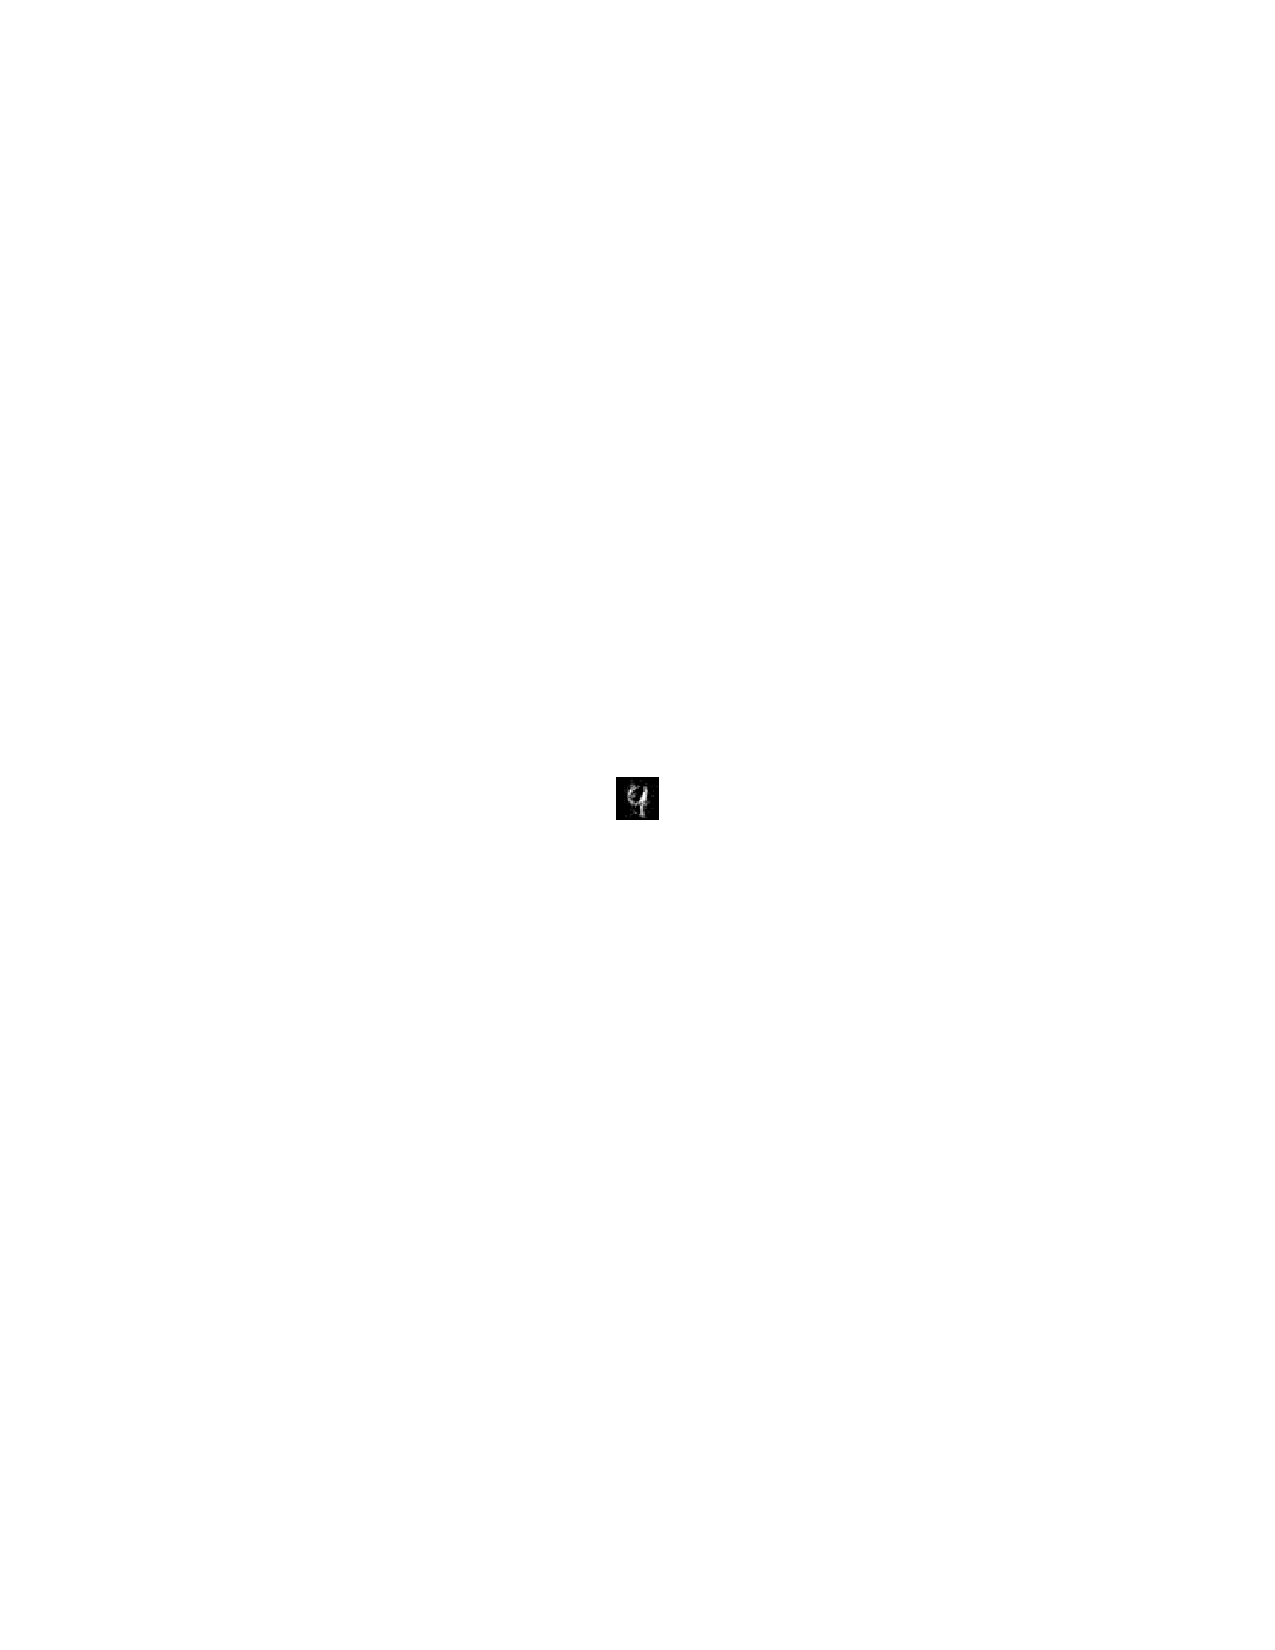
\includegraphics[width =0.9\linewidth, trim = 300 400 300 375, clip]{figs/papernot9pca.pdf}
\end{minipage}
\caption{From left to right, the figures are: original image, adversarial image with FGS method, adversarial image with FGS method and PCA feature reduction, adversarial image with Papernot method, adversarial image with Papernot method and PCA.}\label{fig:picof9s}
\end{figure}